\documentclass[times]{article}

\usepackage[margin=1.0in]{geometry}
\usepackage{graphicx}
\usepackage{adjustbox}
\usepackage{float}
\usepackage{placeins}
\usepackage[none]{hyphenat}
\usepackage{amsmath}
\usepackage[us]{datetime}
\usepackage[explicit]{titlesec}
\begin{document}
	\title{CS 5001 Deep Learning - Fall 2017 \\ Homework 1}
	\author{Dalton Cole}
	\date{\formatdate{12}{10}{2017}}
	\maketitle

	With initial weights $w_0 = 2200$ and $w_1 = 200$ and employing linear regression with one variable yields the results shown in Table \ref{tab:results}.

	As can be seen in Figure \ref{fig:plot}, the linear regression line follows the general trend of the points.

	\begin{table}
		\centering
		\caption{Linear Regression Results}
		\label{tab:results}
		\begin{tabular}{| c | c |}
			\hline
			Learning rate & .001 \\
			\hline
			Number of Iterations & 1500 \\
			\hline
			Sum of Squares Error & 133,987,898 \\
			\hline
			\multicolumn{2}{|c|}{Initial Weights} \\
			\hline
			$w_0$ & 2200 \\
			\hline
			$w_1$ & 200 \\
			\hline
			\multicolumn{2}{|c|}{Final Weights} \\
			\hline
			$w_0$ & 2211.771589 \\
			\hline
			$w_1$ & 234.991411 \\
			\hline
		\end{tabular}
	\end{table}
	

	\begin{figure}
		\caption{Linear Regression with Original Points}
		\label{fig:plot}
		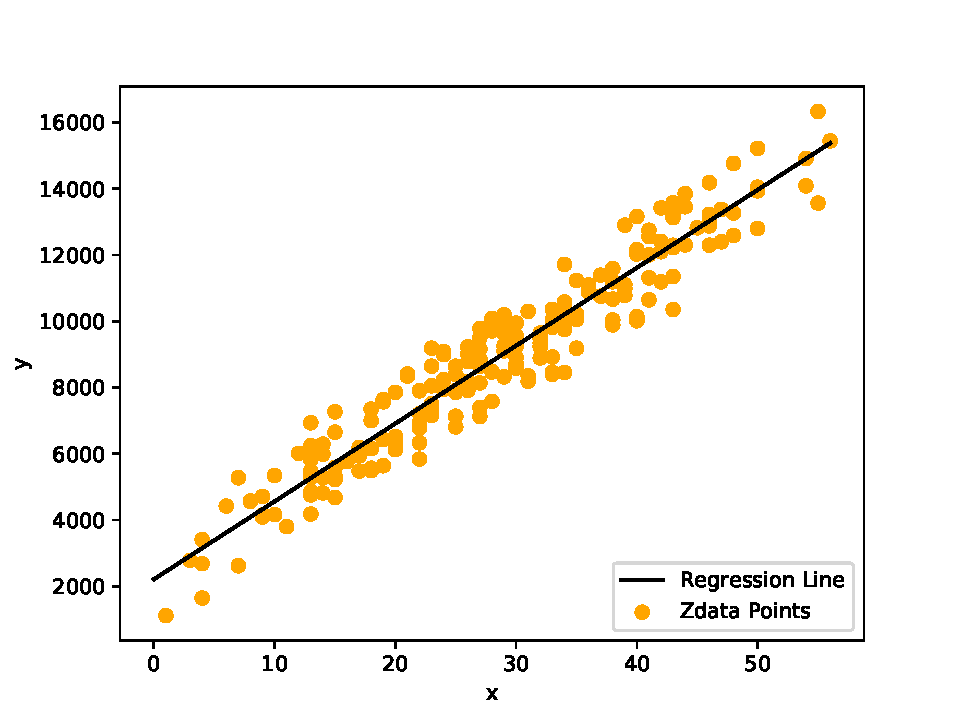
\includegraphics[width=\textwidth]{plot.pdf}
	\end{figure}

	
		
\end{document}